\section{self-replicating malware, generally}

\usetikzlibrary{calc}

\begin{frame}{self-replicating malware}
    \begin{itemize}
    \item attacker's problem: \\getting malware to \myemph{run where they want}
    \item some options:
    \vspace{.5cm}
    \item connect to machine and install it there
    \item send to someone
    \item convince someone else to send it to someone
    \end{itemize}
    \begin{tikzpicture}[overlay,remember picture]
        \begin{visibleenv}<2>
        \node[draw,red!80!black,thick] at ([yshift=1cm]current page.south) {
            \large all automatable!
        };
        \end{visibleenv}
    \end{tikzpicture}
\end{frame}

\begin{frame}<1>{recall: kinds of malware}
    \begin{itemize}
    \item viruses --- infects \myemph{other programs}
    \item \myemph<3>{worms} --- own malicious programs
    \item \myemph<4>{trojans} --- useful (looking) program that also is malicious
    \item \myemph<2>{rootkit} --- silent control of system
    \end{itemize}
    \begin{tikzpicture}[overlay,remember picture]
        \begin{visibleenv}<2>
        \node[draw,red!80!black,thick] at ([yshift=1cm]current page.south) {
            only useful after compromising
        };
        \end{visibleenv}
        \begin{visibleenv}<3>
        \node[draw,red!80!black,thick,align=left] at ([yshift=1cm]current page.south) {
            needs to way to be run in the first place
        };
        \end{visibleenv}
        \begin{visibleenv}<3>
        \node[draw,red!80!black,thick] at ([yshift=1cm]current page.south) {
            targeted ``social engineering''
        };
        \end{visibleenv}
    \end{tikzpicture}
\end{frame}



% FIXME: aside on non-self-replicating malware issues coming up
    % stealth
    % detection

\section{virus: hide in existing programs}

\subsection{motivation}

\begin{frame}{viruses: hiding in files}
    \begin{itemize}
    \item get someone run your malware?
    \item program \myemph{they already want to run}
    \vspace{.5cm}
    \item to spread your malware?
    \item program \myemph<1-2>{they already want to copy}
    \vspace{.5cm}
    \item trojan approach: create/modify new program
    \item simpler: modify already used/shared program
    \end{itemize}
\end{frame}

\begin{frame}{viruses: infecting programs?}
    \begin{itemize}
    \item viruses infecting other programs seems less common
        \begin{itemize}
        \item (but hard to get good statistics\ldots)
        \end{itemize}
    \vspace{.5cm}
    \item but producing infected versions of legitimate software is common
        \begin{itemize}
        \item e.g. fake download site
        \end{itemize}
    \item techniques for automated infection similar to manual infection
    \end{itemize}
\end{frame}


\subsection{early prevalance/motivations}

\begin{frame}[fragile,label=commercial]{virus prevalence}
    \begin{itemize}
        \item viruses \myemph{on commerically sold software media}
        \item from 1990 memo by Chris McDonald:
\begin{Verbatim}[fontsize=\fontsize{8}{9}\selectfont]
4.  MS-DOS INFECTIONS

SOFTWARE                REPORTING LOCATION      DATE     VIRAL INFECTION

a.  Unlock Masterkey    Kennedy Space Center    Oct 89   Vienna
b.  SARGON III          Iceland                 Sep 89   Cascade (1704)
c.  ASYST RTDEMO02.EXE  Fort Belvoir            Aug 89   Jerusalem-B
d.  Desktop Fractal     Various                 Jan 90   Jerusalem (1813)
	Design System
e.  Bureau of the       Government Printing     Jan 90   Jerusalem-B
    Census, Elec. County   Office/US Census Bureau
    & City Data Bk., 1988
f.  Northern Computers  Iceland                 Mar 90   Disk Killer
    (PC Manufacturer shipped infected systems.)
5.  MACINTOSH INFECTIONS

    SOFTWARE            REPORTING LOCATION      DATE     VIRAL INFECTION

a.  NoteWriter          Colgate College         Sep 89   Scores and nVIR
.......
\end{Verbatim}
    \end{itemize}
\imagecredit{https://groups.google.com/forum/\#!original/comp.virus/XJCfYR9T6nI/azflHz5goooJ}
\end{frame}


\begin{frame}{early virus motivations}
    \begin{itemize}
        \item lots of (but not all) early virus software was ``for fun''
        \item not trying to monetize malware
            \begin{itemize}
            \item (like is common today)
            \end{itemize}
        \item hard: Internet connections uncommon
    \end{itemize}
\end{frame}





% FIXME: later prevalence

\section{case study: Vienna}

\begin{frame}{Case Study: Vienna Virus}
\begin{itemize}
    \item Vienna: virus from the 1980s
    \item This version: published in Ralf Burger, ``Computer Viruses: a high-tech disease'' (1988)
    \item targetted COM-format executables on DOS
\end{itemize}
\end{frame}




\subsection{aside: COM files}


\begin{frame}{Diversion: .COM files}
    \begin{itemize}
    \item .COM is a \myemph{very simple} executable format
    \item no header, no segments, no sections
    \item file contents loaded at fixed address {\tt 0x0100}
    \item execution starts at {\tt 0x0100}
    \item everything is read/write/execute (no virtual memory)
    \end{itemize}
\end{frame}




\subsection{entry/exit}

\usetikzlibrary{calc}

\begin{frame}[fragile,label=vienna]{Vienna: infection}
\lstset{
    language=myasm,
    style=smaller,
    moredelim={**[is][\btHL<2>]{~hi2~}{~endhi2~}},
}
\begin{tikzpicture}
\tikzset{programBox/.style={draw,thick},every label/.style={inner sep=1mm,outer sep=0mm}}
\node[programBox,minimum height=3cm,label={north:uninfected},anchor=north west] (uninfect) at (0,0) {
\begin{lstlisting}
0x0100:
    ~hi2~mov $0x4f28, %cx~endhi2~
    /* b9 28 4f */
0x0103:
    mov $0x9e4e, %si
    /* be 4e 9e */
    mov %si, %di
    push %ds
    /* more normal
       program
       code */
....
0x0700: /* end */

\end{lstlisting}
};
\node[overlay,programBox,anchor=north west,label={[overlay]north:infected}] at ([yshift=.5cm,xshift=1cm]uninfect.north east) {
\begin{lstlisting}
0x0100: jmp 0x0700
0x0103: mov $0x9e4e, %si
...
0x0700:
    push %cx
    ... // %si <- 0x903
    mov $0x100, %di
    mov $3, %cx
    rep movsb
    ...
    mov $0x0100, %di
    push %di
    xor %di, %di
    ret
...
0x0903:
    ~hi2~.bytes 0xb9 0x28 0x4f~endhi2~
...
\end{lstlisting}
};
\end{tikzpicture}
\end{frame}

\begin{frame}[fragile,label=viennaFixup]{Vienna: ``fixup''}
\lstset{
    language=myasm,
    style=small,
    moredelim={**[is][\btHL<2>]{~hi2~}{~endhi2~}},
    moredelim={**[is][\btHL<3>]{~hi3~}{~endhi3~}},
}
\begin{lstlisting}
0x0700:
    push %cx // initial value of %cx matters??
    mov ~hi3~$0x8fd~endhi3~, %si // %si <- beginning of data
    mov %si, %dx // save %si
        // movsb uses %si, so
        // can't use another register
    add $0xa, %si // offset of saved code in data
    mov $0x100, %di // target address
    mov $3, %cx // bytes changed
    /* copy %cx bytes from (%si) to (%di) */
    rep movsb 
    ...
...
// saved copy of original application code
0x903: ~hi2~.byte 0xb9 .byte 0x28 .byte 0x4f~endhi2~
\end{lstlisting}
\end{frame}

\begin{frame}[fragile,label=viennaReturn]{Vienna: return}
\lstset{language=myasm,style=small}
\begin{lstlisting}
0x08e7:
    pop %cx // restore initial value of %cx, %sp
    xor %ax, %ax // %ax <- 0
    xor %bx, %bx
    xor %dx, %dx
    xor %si, %si
    // push 0x0100
    mov $0x0100, %di
    push %di 
    xor %di, %di // %di <- 0
    // pop 0x0100 from stack
    // jmp to 0x0100
    ret 
\end{lstlisting}
\begin{itemize}
\item<1> question: why not just jmp 0x0100 ?
\end{itemize}
\end{frame}



\subsection{infection outline}


\begin{frame}<1>[label=viennaOutline]{Vienna: infection outline}
\begin{itemize}
\item Vienna \myemph{appends} code to infected application
\vspace{.5cm}
\item \myemph<2>{where does it read the code come from?}
\item \myemph<3>{how is code adjusted for new location in the binary?}
    \begin{itemize}\item what linker would do\end{itemize}
\item \myemph<4>{how does it keep files from getting infinitely long?}
\end{itemize}
\end{frame}


\subsection{writing your own code?}

\againframe<2>{viennaOutline}
\subsubsection{aside: quines}


\begin{frame}{quines}
\begin{itemize}
    \item exercise: write a C program that outputs its source code
        \begin{itemize}
        \item (pseudo-code only okay)
        \end{itemize}
    \item possible in any {\small (Turing-complete)} programming language
    \item called a ``quine''
\end{itemize}
\end{frame}

\begin{frame}[fragile,label=quineClever]{clever quine solution}
\lstset{language=C,style=small,
    moredelim={**[is][\btHL<2|handout:0>]{@hi2@}{@endhi@}},
    moredelim={**[is][\btHL<3|handout:0>]{@hi3@}{@endhi@}},
    showstringspaces=false,
}
\begin{lstlisting}
#include <stdio.h>
char*x="int main(){
       `\btHL<2>{printf(p,10,34,x,34,10,34,p,34,10,x,10);}`
       }";
@hi3@char*p@endhi@="#include <stdio.h>%c
    char*x=%c%s%c;%cchar*p=%c%s%c;
    %c%s%c";
int main(){
    @hi2@printf(p,10,34,x,34,10,34,p,34,10,x,10);@endhi@
}
\end{lstlisting}
\begin{itemize}
\item some line wrapping for readability --- shouldn't be in actual quine
\end{itemize}
\begin{tikzpicture}[overlay,remember picture]
    \begin{visibleenv}<2|handout:0>
        \node[fill=white,draw,thick,align=left] at (current page.center) {
            {\tt printf} to fill template: \\
            {\tt 10} = newline; {\tt 34} = double-quote; \\
            {\tt x}, {\tt p} = template/constant strings
        };
    \end{visibleenv}
    \begin{visibleenv}<3|handout:0>
        \node[fill=white,draw,thick,align=left] at ([yshift=1cm]current page.center) {
            template filled by printf
        };
    \end{visibleenv}
\end{tikzpicture}
\end{frame}

\begin{frame}[fragile,label=quineDumb]{dumb quine solution}
\begin{lstlisting}[language=C,style=small]
#include <stdio.h>
int main(void) {
    char buffer[1024];
    FILE *f = fopen("quine.c", "r");
    size_t bytes = fread(buffer, 1,
                         sizeof(buffer), f);
    fwrite(buffer, 1, bytes, stdout);
    return 0;
}
\end{lstlisting}
\begin{itemize}
\item a lot more straightforward!
\item but ``cheating''
\end{itemize}
\end{frame}



\subsubsection{Vienna replication code}


\begin{frame}[fragile,label=virusWriting]{Vienna copying}
\lstset{
    style=small,
    language=myasm,
    moredelim={**[is][\btHL<2|handout:0>]{@hi2@}{@endhi@}},
}
\begin{lstlisting}
@hi2@mov $0x8f9, %si@endhi@ // %si = beginning of virus data
...
mov $0x288, %cx // length of virus
mov $0x40, %ah  // system call # for write
mov %si, %dx
sub $0x1f9, %dx // %dx = beginning of virus code
int 0x21 // make write system call
\end{lstlisting}
\end{frame}




\subsection{Vienan relocation code}
% FIXME: need to explain why this is a problem
\againframe<3>{viennaOutline}

\subsubsection{Vienna's relocation code}

\begin{frame}[fragile,label=virusReloc2]{Vienna relocation}
\lstset{
    style=small,
    language=myasm,
    moredelim={**[is][\btHL<1|handout:0>]{@hi1@}{@endhi@}},
    moredelim={**[is][\btHL<2|handout:0>]{@hi2@}{@endhi@}},
    moredelim={**[is][\btHL<3|handout:0>]{@hi3@}{@endhi@}},
}
\begin{lstlisting}
// set virus data address:
0x700: @hi1@mov $0x8f9, %si@endhi@
       // machine code: be f9 08
       // be: opcode
       // f9 08: immediate
...
// %ax contains file length (of file to infect)
mov %ax, %cx
...
@hi3@add $0x2f9, %cx@endhi@
mov %si, %di   
sub $0x1f7, %di // %di <- 0x701
@hi2@mov %cx, (%di)@endhi@  // update mov instruction
...
\end{lstlisting}
\begin{tikzpicture}[overlay,remember picture]
\begin{visibleenv}<1>
\node[align=left,draw,very thick,fill=white] at (current page.center) {
    Vienna design: need to access global variables, etc. \\
    solution: base pointer for virus data \\
    problem: location changes depending on where virus is
};
\end{visibleenv}
\end{tikzpicture}
\end{frame}

\begin{frame}[fragile,label=virusReloc3]{Vienna relocation}
\begin{itemize}
\item edit actual code for {\tt mov}
\item why doesn't this disrupt virus execution?
    \begin{itemize}\item<2> already ran that instruction\end{itemize}
\end{itemize}
\end{frame}

\begin{frame}[fragile,label=virusReloc4]{Vienna relocation}
\lstset{
    style=smaller,
    language=myasm,
    moredelim={**[is][\btHL<2|handout:0>]{@hi2@}{@endhi@}},
    moredelim={**[is][\btHL<3|handout:0>]{@hi3@}{@endhi@}},
}
\begin{lstlisting}
0x700: mov $0x8f9, %si
...
// %ax contains file length
//     (of file to infect)
mov %ax, %cx
sub $3, %ax
// update template jmp instruction
mov %ax, @hi2@0xe(%si)@endhi@ // 0xe + %si = 0x907
...
mov $40, %ah
mov $3, %cx
mov %si, %dx  
add $0xD, @hi3@%dx@endhi@ // dx <- 0x906
int 0x21 // system call: write 3 bytes from 0x906
...
0x906: @hi2@e9 fd 05@endhi@ // jmp PC+FD 05
\end{lstlisting}
\end{frame}



\subsubsection{alternate: PIC}

\begin{frame}[fragile,label=altVirusReloc]{alternative relocation}
    \begin{itemize}
    \item could avoid having pointer to update:
    \end{itemize}
\begin{Verbatim}[fontsize=\fontsize{10}{11}\selectfont,commandchars=Q\{\}]
0000000000000000 <next-0x3>:
   0:   e8 Qtextbf{00 00}                call   3 <next>
    Qtextit{target addresses encoded relatively}
    Qtextit{pushes return address (next) onto stack}
0000000000000003 <next>:
   3:   59                      pop    %cx
    Qtextit{cx containts address of the pop instruction}
\end{Verbatim}
    \begin{itemize}
    \item why didn't Vienna do this?
    \end{itemize}
\end{frame}



\subsection{avoiding reinfection}
\againframe<4>{viennaOutline}

% FIXME: reflection on Vienna detection/portability
    % preview of future topics
        % looking for virus patterns that won't appear in executables

% FIXME: copy intro

\section{viruses: where to put code}


\begin{frame}{where to put code}
    \begin{itemize}
    \item viruses insert code in other programs
    \item Vienna's choice: end of executables
    \item search for \texttt{.COM} executables on system
    \vspace{.5cm}
    \item considerations for other options:
    \item spreading: identifying useful files to infect
        \begin{itemize}
        \item will be copied elsewhere?
        \item will be run?
        \end{itemize}
    \item stealth: avoiding detection
        \begin{itemize}
        \item Vienna: file size changes --- easy to find?
        \item Vienna: weird modification time --- easy to find?
        \end{itemize}
    \end{itemize}
\end{frame}

\begin{frame}<1>[label=whereCode]{where to put code: options}
    \begin{itemize}
    \item one \textit{or more} of:
    \item \myemph<2>{replacing executable code}
    \item \myemph<3>{after executable code (Vienna)}
    \item \myemph<4>{in unused executable code}
    \item \myemph<5>{inside OS code}
    \item \myemph<6>{in memory}
    \item \myemph<7>{replace existing code}
    \end{itemize}
\end{frame}



\subsection{replacing executables?}

\againframe<2>{whereCode}

\usetikzlibrary{arrows.meta}

\begin{frame}{replace executable}
    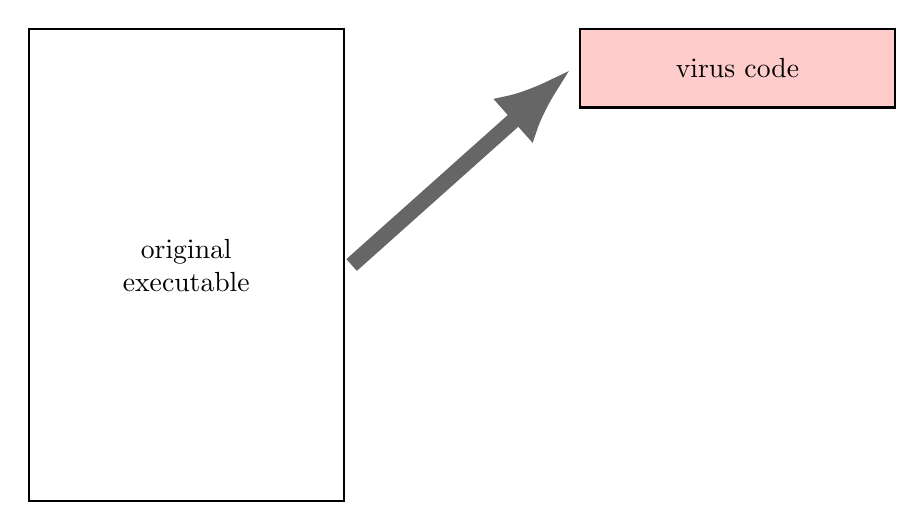
\begin{tikzpicture}
    \draw[thick] (0, 0) rectangle (4, -6) node[midway,align=center] {original\\executable};
    \draw[line width=2mm,-Latex,black!60] (4.1, -3) -- (6.9, -.5);
    \begin{scope}[xshift=7cm]
    \draw[thick,fill=red!20] (0, 0) rectangle (4, -1) node[midway,align=center] {virus code};
    \end{scope}
    \end{tikzpicture}
\end{frame}

\begin{frame}{replace executable?}
    \begin{itemize}
    \item seems silly --- not stealthy!
    \item has appeared in the wild --- ILOVEYOU
    \item 2000 ILOVEYOU Worm
        \begin{itemize}
        \item written in Visual Basic (!)
        \item spread via email
        \item replaced lots of files with copies of itself
        \end{itemize}
    \item huge impact --- because destroying data to copy itself
    \end{itemize}
\end{frame}

\begin{frame}{replace executable --- subtle}
    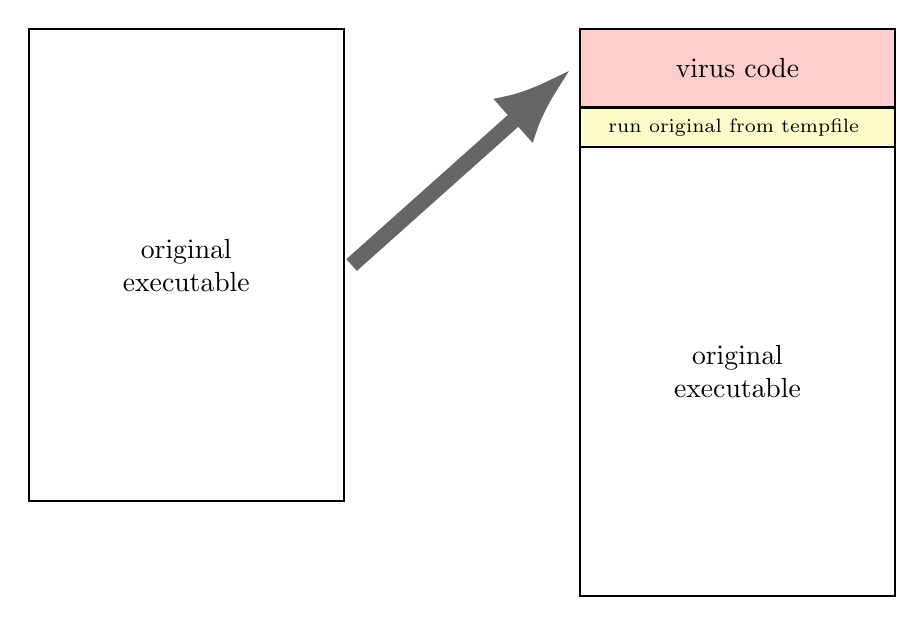
\begin{tikzpicture}
    \draw[thick] (0, 0) rectangle (4, -6) node[midway,align=center] {original\\executable};
    \draw[line width=2mm,-Latex,black!60] (4.1, -3) -- (6.9, -.5);
    \begin{scope}[xshift=7cm]
    \draw[thick,fill=red!20] (0, 0) rectangle (4, -1) node[midway,align=center] {virus code};
    \draw[thick,fill=yellow!20] (0, -1) rectangle (4, -1.5) node[midway,align=center,font=\scriptsize] {
        run original from tempfile
    };
    \draw[thick] (0, -1.5) rectangle (4, -7.2) node[midway,align=center] {original\\executable};
    \end{scope}
    \end{tikzpicture}
\end{frame}



\subsection{appending/compressing}

% FIXME: good place for aside on modern executable formats

\againframe<3>{whereCode}

\usetikzlibrary{arrows.meta,patterns}
\begin{frame}{appending}
    \pdftooltip{
    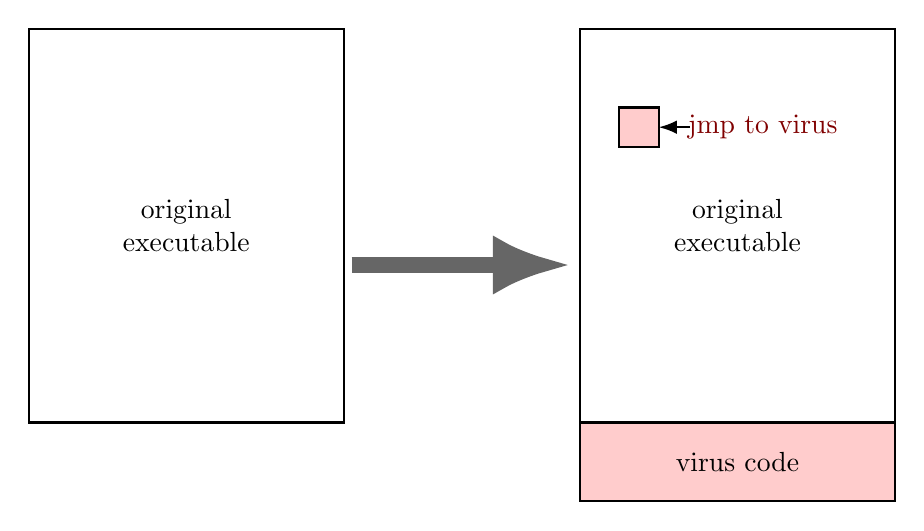
\begin{tikzpicture}
    \draw[thick] (0, 0) rectangle (4, -5) node[midway,align=center] {original\\executable};
    \draw[line width=2mm,-Latex,black!60] (4.1, -3) -- (6.9, -3);
    \begin{scope}[xshift=7cm]
    \draw[thick] (0, 0) rectangle (4, -5) node[midway,align=center] {original\\executable};
    \draw[fill=red!20,thick] (0, -5) rectangle (4, -6)
        node[midway,align=center] {virus code};
    \draw[fill=red!20,thick] (0.5, -1) rectangle (1, -1.5);
    \node[anchor=west,red!50!black] at (1.25, -1.25) {jmp to virus};
    \draw[thick,Latex-] (1, -1.25) -- (1.4, -1.25);
    \end{scope}
    \end{tikzpicture}
    }{executable transformed by replacing some of the original code with jmp + appending virus}
\end{frame}

\begin{frame}{appending and executable formats}
    \begin{itemize}
    \item COM files are very simple --- no metadata
    \item modern executable formats have length information to update:
    \vspace{.5cm}
    \item option 1: add segment (ELF LOAD) to program header
        \begin{itemize}
        \item (often a little extra space after program header, due to page-alignment)
        \end{itemize}
    \item option 2: update last segment of program header
        \begin{itemize}
        \item change its size
        \item make it executable if it isn't (and often not --- often data)
        \end{itemize}
    \end{itemize}
\end{frame}





\subsection{cavaties}

\againframe<4>{whereCode}

\begin{frame}{unused code???}
    \begin{itemize}
    \item why would a program have unused code????
    \end{itemize}
\end{frame}

\begin{frame}[fragile,label=lsStudy1]{unused code case study: /bin/ls}
    \begin{itemize}
    \item unreachable no-ops!
    \end{itemize}
\begin{Verbatim}[fontsize=\fontsize{9}{10}\selectfont,commandchars=Q\{\}]
...
  403788:	e9 59 0c 00 00       	jmpq   4043e6 <__sprintf_chk@plt+0x1a06>
  Qtextbf{40378d:	0f 1f 00             	nopl   (%rax)}
  403790:	ba 05 00 00 00       	mov    $0x5,%edx
...
  403ab9:	eb 4d                	jmp    403b08 <__sprintf_chk@plt+0x1128>
  Qtextbf{403abb:	0f 1f 44 00 00       	nopl   0x0(%rax,%rax,1)}
  403ac0:	4d 8b 7f 08          	mov    0x8(%r15),%r15
...
  404a01:	c3                   	retq   
  Qtextbf{404a02:	0f 1f 40 00          	nopl   0x0(%rax)}
  Qtextbf{404a06:	66 2e 0f 1f 84 00 00 	nopw   %cs:0x0(%rax,%rax,1)}
  Qtextbf{404a0d:	00 00 00 }
  404a10:	be 00 e6 61 00       	mov    $0x61e600,%esi
...
\end{Verbatim}
\end{frame}

\begin{frame}{why empty space?}
\begin{itemize}
\item Intel Optimization Reference Manual: \\
``\textbf{Assembly/Compiler Coding Rule 12. (M impact, H generality)} \\All branch targets should be 16-byte aligned.''
\begin{itemize}
    \item better for instruction cache {\small (and TLB and related caches)}
    \item better for instruction decode logic
    \item function calls, jumps count as branches for this purpose
\end{itemize}
\end{frame}

\begin{frame}{why weird nops}
    \begin{itemize}
    \item could fill with \myemph{anything} --- unreachable
    \item some platforms: filled with crashing instructions
    \vspace{.5cm}
    \item why not in example? assembler just told to align instruction
        \begin{itemize}
        \item not told previous instruction was jump/ret/etc. \ldots
        \item and assembler doesn't bother checking
        \end{itemize}
    \item probably better for CPU to fill with some instruction; Intel manual:
        \begin{itemize}
        \item ``Placing data immediately following an indirect branch
              can cause performance problems. If the data consists of all zeros,
              it looks like a long stream of ADDs to memory destinations, and this can cause
              resource conflicts\ldots''
        \end{itemize}
    \end{itemize}
\end{frame}

\begin{frame}<1>[label=otherSpace]{other empty space}
\begin{itemize}
\item \myemph<2>{unused dynamic linking structure}
\item \myemph<3>{unused space between segments}
\item unused debugging/symbol table information?
\item unused header space 
    \begin{itemize}
    \item file offsets of segments can be in middle of header
    \item loader doesn't care what segments ``mean''
    \end{itemize}
\end{itemize}
\end{frame}

\againframe<2>{otherSpace}

\begin{frame}[label=spaceDyn,fragile]{dynamic linking cavity}
\begin{itemize}
\item {\tt .dynamic} section --- data structure used by dynamic linker:
\item format: list of 8-byte type, 8-byte value
    \begin{itemize}
    \item terminated by type == 0 entry
    \end{itemize}
\end{itemize}
\begin{Verbatim}[fontsize=\fontsize{9}{10}\selectfont,commandchars=Q\{\}]
Contents of section .dynamic:
 600e28 01000000 00000000 01000000 00000000  ................
    Qtextit{... several non-empty entries ...}
 600f88 f0ffff6f 00000000 56034000 00000000  ...o....V.@.....
    Qtextit{VERSYM (required library version info at) 0x400356}
 600f98 Qtextit{00000000 00000000 00000000 00000000}  ................
    Qtextit{NULL --- end of linker info}
 600fa8 Qtextbf{00000000 00000000 00000000 00000000}  ................
    Qtextit{unused! (and below)}
 600fb8 Qtextbf{00000000 00000000 00000000 00000000}  ................
 600fc8 Qtextbf{00000000 00000000 00000000 00000000}  ................
 600fd8 Qtextbf{00000000 00000000 00000000 00000000}  ................
 600fe8 Qtextbf{00000000 00000000 00000000 00000000}  ................
\end{Verbatim}
\end{frame}





\subsubsection{chaining cavaties (CIH case study)}

\usetikzlibrary{arrows.meta,patterns}

\begin{frame}{is there enough empty space?}
\begin{itemize}
    \item cavities look awfully small
    \item really small viruses?
    \item solution: chain cavities tgoether
\end{itemize}
\end{frame}

\begin{frame}{case study: CIH (1)}
    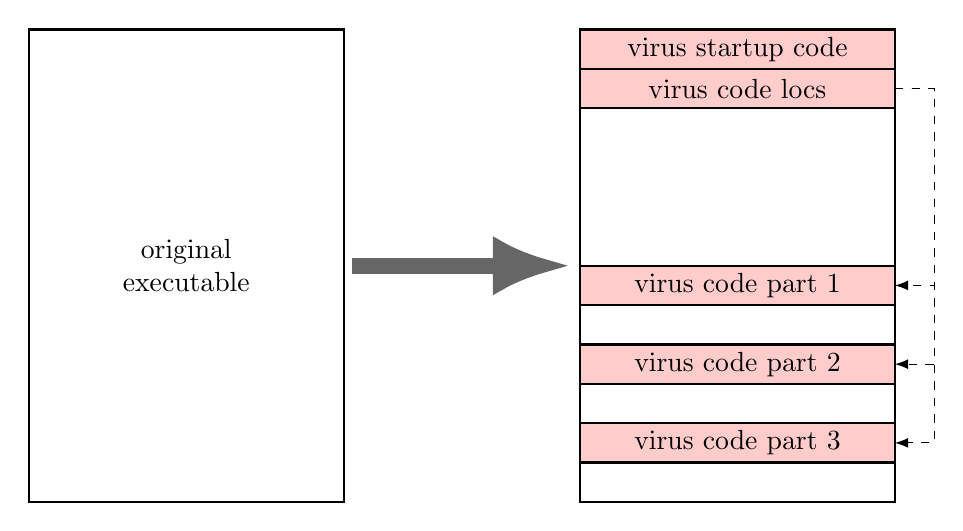
\begin{tikzpicture}
    \draw[thick] (0, 0) rectangle (4, -6) node[midway,align=center] {original\\executable};
    \draw[line width=2mm,-Latex,black!60] (4.1, -3) -- (6.9, -3);
    \begin{scope}[xshift=7cm]
    \draw[fill=red!20,thick] (0, 0) rectangle (4, -0.5) node[midway] {virus startup code};
    \draw[fill=red!20,thick] (0, -0.5) rectangle (4, -1) node[midway] {virus code locs};
    \draw[thick] (0, -1) rectangle (4, -6);
    \draw[fill=red!20,thick] (0, -3) rectangle (4, -3.5)
        node[midway] {virus code part 1};
    \draw[fill=red!20,thick] (0, -4) rectangle (4, -4.5)
        node[midway] {virus code part 2};
    \draw[fill=red!20,thick] (0, -5) rectangle (4, -5.5)
        node[midway] {virus code part 3};
    \draw[dashed,thin,-Latex] (4, -0.75) -- (4.5, -0.75) |- (4, -3.25);
    \draw[dashed,thin,-Latex] (4, -0.75) -- (4.5, -0.75) |- (4, -4.25);
    \draw[dashed,thin,-Latex] (4, -0.75) -- (4.5, -0.75) |- (4, -5.25);
    \end{scope}
    \end{tikzpicture}
\end{frame}

\begin{frame}{case study: CIH (2)}
    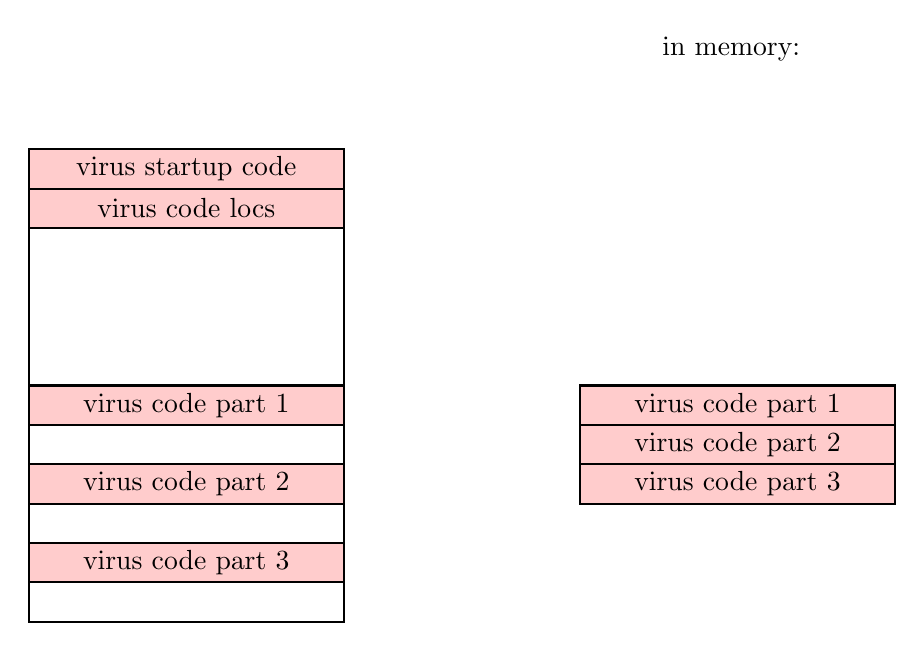
\begin{tikzpicture}
    \draw[fill=red!20,thick] (0, 0) rectangle (4, -0.5) node[midway] {virus startup code};
    \draw[fill=red!20,thick] (0, -0.5) rectangle (4, -1) node[midway] {virus code locs};
    \draw[thick] (0, -1) rectangle (4, -6);
    \draw[fill=red!20,thick] (0, -3) rectangle (4, -3.5)
        node[midway] {virus code part 1};
    \draw[fill=red!20,thick] (0, -4) rectangle (4, -4.5)
        node[midway] {virus code part 2};
    \draw[fill=red!20,thick] (0, -5) rectangle (4, -5.5)
        node[midway] {virus code part 3};
    \begin{scope}[xshift=7cm]
        \node[align=center,anchor=south] at (2, 1) { in memory: };
        \draw[fill=red!20,thick] (0, -3) rectangle (4, -3.5)
            node[midway] {virus code part 1};
        \draw[fill=red!20,thick] (0, -3.5) rectangle (4, -4)
            node[midway] {virus code part 2};
        \draw[fill=red!20,thick] (0, -4) rectangle (4, -4.5)
            node[midway] {virus code part 3};
    \end{scope}
    \end{tikzpicture}
\end{frame}

\begin{frame}{CIH cavities}
    \begin{itemize}
    \item gaps between sections
        \begin{itemize}
        \item common Windows linker aligned sections
        \item (align = start on address multiple of $N$, e.g. $4096$)
        \end{itemize}
    \item reassembling code avoids worrying about splitting instructions
    \end{itemize}
\end{frame}



\subsection{boot sector}

\againframe<5>{whereCode}

\usetikzlibrary{arrows.meta,chains}

\begin{frame}<1-2>[label=bootProc]{boot process}
    \begin{tikzpicture}
        \begin{scope}[start chain=going below,every node/.style={draw,align=center,join,on chain,thick,minimum width=3.5cm},
                      every join/.style={-Latex,thick}]
        \node[draw=none] (fixedLoc) { processor reset };
        \node[alt=<3>{draw=red,very thick}{}] (bios) {BIOS/EFI \\ \small (chip on motherboard)};
        \node[alt=<2>{draw=red,very thick}{}] (bootloader) {bootloader};
        \node[alt=<4>{draw=red,very thick}{}] (os) {operating system};
        \end{scope}
        \node[left=.5cm of bios,font=\small] (biosLabel) {very CPU/motherboard-specific code};
        \draw[-Latex,thick] (biosLabel) -- (bios);
        \node[left=.5cm of bootloader,font=\small,align=right] (bootloaderLabel) {fixed location on disk \\ code that understands files};
        \draw[-Latex,thick] (bootloaderLabel) -- (bootloader);
        \node[left=.5cm of os,font=\small] (osLabel) {files in a filesystem};
        \draw[-Latex,thick] (osLabel) -- (os);
    \end{tikzpicture}
\end{frame}

\begin{frame}{bootloaders in the DOS era}
    \begin{itemize}
    \item used to be common to boot from floppies
    \item \myemph{default to booting from floppy} if present
        \begin{itemize}
        \item even if hard drive to boot from
        \end{itemize}
    \item applications distributed as bootable floppies
    \item so bootloaders on all devices were a target for viruses
    \end{itemize}
\end{frame}

\begin{frame}{historic bootloader layout}
    \begin{itemize}
    \item bootloader in \myemph{first sector} (512 bytes) of device
    \item (along with partition information)
    \item code in BIOS to copy bootloader into RAM, start running
    \item bootloader responsible for disk I/O etc.
        \begin{itemize}
        \item some library-like functionality in BIOS for I/O
        \end{itemize}
    \end{itemize}
\end{frame}

\begin{frame}{bootloader viruses}
    \newcommand{\tearBox}{
        \draw[very thick] (0, -6) -- (0, 0) -- (4, 0) -- (4, -6);
        \draw[thick] (0, -6) -- (1.2, -5.5) -- (2., -6.6) -- (2.6, -5.8) -- (3.5, -6.6) -- (4, -6);
    }
    \begin{itemize}
    \item example: Stoned
    \end{itemize}
    \begin{tikzpicture}
        \draw[fill=green!20] (0, 0) rectangle (4, -.2);
        \draw[fill=yellow!20] (0, -.2) rectangle (4, -0.5) node[midway,font=\tiny] { partition table };
        \draw[fill=green!20] (0, -.5) rectangle (4, -1.0) node[midway,font=\small] { bootloader };
        \tearBox
        \begin{scope}[xshift=7cm]
        \draw[fill=red!20] (0, 0) rectangle (4, -.2);
        \draw[fill=yellow!20] (0, -.2) rectangle (4, -0.5) node[midway,font=\tiny] { partition table };
        \draw[fill=red!20] (0, -.5) rectangle (4, -1.0) node[midway,font=\small] { virus code };
        \begin{scope}[yshift=-4cm]
        \draw[fill=green!20] (0, 0) rectangle (4, -.2);
        \draw[fill=green!20] (0, -.5) rectangle (4, -1.0) node[midway,font=\small] { saved bootloader };
        \draw[dashed,fill=yellow!20] (0, -.2) rectangle (4, -0.5) node[midway,font=\tiny] { partition table (unused) };
        \end{scope}
        \tearBox 
        \end{scope}
        \draw[line width=1mm,black!50, -Latex] (4.2, -3) -- (6.8, -3);

        \begin{pgfonlayer}{bg}
            \begin{visibleenv}<2>
                \path[fill=blue!30] (0, -4) rectangle (4, -5) node[midway] { data here??? };
            \end{visibleenv}
        \end{pgfonlayer}
    \end{tikzpicture}
\end{frame}

\begin{frame}{data here???}
    \begin{itemize}
        \item might be data there --- risk
        \item some unused space after partition table/boot loader common
            \begin{itemize}
            \item (allegedly)
            \end{itemize}
        \item also be filesystem metadata not used on smaller floppies/disks
        \vspace{.5cm}
        \item but could be wrong --- oops
    \end{itemize}
\end{frame}

\begin{frame}{modern bootloaders --- UEFI}
    \begin{itemize}
    \item BIOS-based boot is going away (slowly)
    \item new thing: UEFI (Universal Extensible Firmware Interface)
    \item like BIOS:
        \begin{itemize}
        \item library functionality for bootloaders
        \item loads initial code from disk/DVD/etc.
        \end{itemize}
    \item unlike BIOS:
        \begin{itemize}
        \item much more understanding of file systems
        \item much more modern set of library calls
        \end{itemize}
    \end{itemize}
\end{frame}

\againframe<3>{bootProc}

\begin{frame}{BIOS/UEFI implants}
    \begin{itemize}
    \item infrequent
    \item BIOS/UEFI code is \myemph{very non-portable}
    \item BIOS/UEFI update may require physical access
    \item BIOS/UEFI code may require cryptographic signatures
    \item \ldots but \myemph{very hard to remove} --- ``persist'' other malware
    \item reports of BIOS/UEFI-infecting ``implants''
        \begin{itemize}
        \item sold by Hacking Team (Milan-based malware company) 
        \item listed in leaked NSA Tailored Access Group catalog
        \end{itemize}
    \end{itemize}
\end{frame}

\againframe<4>{bootProc}

\begin{frame}{system files}
    \begin{itemize}
    \item simpliest strategy: stuff that runs when you start your computer
    \item add a new startup program, run in the background
        \begin{itemize}
        \item easy to blend in
        \end{itemize}
    \vspace{.5cm}
    \item alternatively, infect one of many system programs automatically run
    \end{itemize}

    % FIXME: example from CodeRed or similar?
\end{frame}

 % FIXME: split out UEFI/Secure Boot section

\subsection{memory residence}


\begin{frame}{memory residence}
    \begin{itemize}
    \item malware wants to keep doing stuff
    \item one option --- background process (easy on modern OSs)
    \item also stealthy options:
        \begin{itemize}
        \item insert self into OS code
        \item insert self into other running programs
        \end{itemize}
    \end{itemize}
\end{frame}
 % FIXME: should have more extensive discussion of this somewhere

\section{virus: getting code invoked}


\begin{frame}<1-2>[label=invokeOptions]{invoking virus code: options}
    \begin{itemize}
    \item boot loader
    \item \myemph<2>{change starting location} 
    \item alternative approaches: ``entry point obscuring''
    \item \myemph<3>{edit code that's going to run anyways}
    \item \myemph<4>{replace a function pointer} (or similar)
    \item \ldots
    \end{itemize}
\end{frame}


\subsection{changing start location}


\begin{frame}[fragile,label=invokeStarting]{starting locations}
\begin{Verbatim}[fontsize=\fontsize{10}{11}\selectfont,commandchars=Q\{\}]
/bin/ls:     file format elf64-x86-64
/bin/ls
architecture: i386:x86-64, flags 0x00000112:
EXEC_P, HAS_SYMS, D_PAGED
start address Qmyemph{0x00000000004049a0}
\end{Verbatim}
    \begin{itemize}
    \item modern executable formats have `starting address' field
    \item just change it, insert jump to old address after virus code
    \end{itemize}
\end{frame}




\subsection{overwrite existing code}

\begin{frame}<1>[fragile,label=runAnyways]{run anyways?}
    \begin{itemize}
    \item add code at start of program (Vienna)
        \begin{itemize}
        \item \myemph<2>{plus restore replaced code after running malware code}
        \end{itemize}
    \item return with padding after it:
\begin{Verbatim}[fontsize=\fontsize{10}{11}\selectfont,commandchars=Q\{\}]
  404a01:       c3                      Qtextbf{retq}
  404a02:       0f 1f 40 00             nopl   0x0(%rax)
                Qtextit{replace with}
  404a01:       e9 XX XX XX XX          Qtextbf{jmpq    YYYYYYY}
\end{Verbatim}
        \begin{itemize}
        \item plus return after running malware code
        \end{itemize}
    \item any random place in program?
        \begin{itemize}
        \item just not in the \myemph{middle of instruction}
        \item and \myemph<2>{replace orignal code after running malware code}
        \end{itemize}
    \end{itemize}
\end{frame}

\begin{frame}[fragile,label=findValidChallenge]{challenge: valid locations}
    \begin{itemize}
    \item x86: probably don't want a full instruction parser
    \item x86: might be non-instruction stuff mixed in with code:
\begin{lstlisting}[language=myasm,style=smaller]
do_some_floating_point_stuff:
            movss float_one(%rip), %xmm0
            ...
            retq
float_one: .float 1
\end{lstlisting}
    \begin{itemize}
        \item floating point value one ({\tt 00 00 80 3f}) is not valid machine code
        \item disassembler might lose track of instruction boundaries
    \end{itemize}
    \end{itemize}
\end{frame}

\begin{frame}[fragile,label=findValidFindFunc]{finding function calls}
    \begin{itemize}
    \item one idea: replace calls
    \item normal x86 call FOO: {\tt E8 \textit{(32-bit value: PC - address of foo)}}
    \item could look for E8 in code --- \myemph{lots of false positives}
        \begin{itemize}
        \item probably even if one excludes out-of-range addresses
        \end{itemize}
    \end{itemize}
\end{frame}

\begin{frame}[fragile,label=findValidFindFunc2]{really finding function calls (1)}
\lstset{language=myasm,style=small}
    \begin{itemize}
    \item e.g. some popular compilers started x86-32 functions with
\begin{lstlisting}
foo:
    push %ebp       // push old frame pointer
    // 0x55
    mov %esp, %ebp  // set frame pointer to stack pointer
    // 0x89 0xec
\end{lstlisting}
    \item use to identify when {\tt e8} refers to real function
    \begin{itemize}
    \item (full version: also have some other function start patterns)
    \end{itemize}
    \end{itemize}
\end{frame}

\begin{frame}{really finding function calls (2)}
    \begin{itemize}
    \item x86-64 assembly seen a lot of ENDBR64 (hex {\tt f3 0f 1e fa})
    \item marker for valid locations to jump to
        \begin{itemize}
        \item intention: part of possible defense against return-oriented-programming-style attacks
        \item (we'll talk about what this means later)
        \end{itemize}
    \item likely only seen at beginning of functions, switch statement cases, etc.
    \end{itemize}
\end{frame}

\againframe<2>{runAnyways}

\begin{frame}{restoring replaced code?}
    \begin{itemize}
    \item Vienna: just write to memory addres
    \vspace{.5cm}
    \item modern OS: segfault/general protection fault
        \begin{itemize}
        \item code loaded read-only
        \end{itemize}
    \item easy solution: make library call to make it writable
        \begin{itemize}
        \item Linux: \texttt{mprotect}
        \item functionality exists to, e.g., allow compiling code at runtime
        \end{itemize}
    \end{itemize}
\end{frame}


\subsection{using dynamic linking features}

\begin{frame}{infecting shared libraries via relocations}
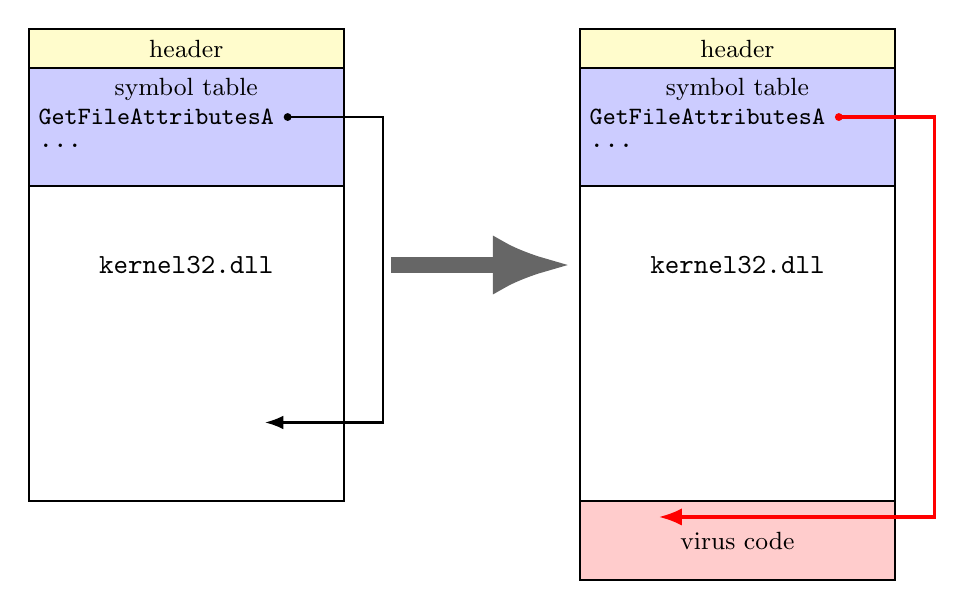
\begin{tikzpicture}
    \draw[thick] (0, 0) rectangle (4, -6) coordinate (bottomRight) node[midway] { \tt kernel32.dll };
    \draw[thick,fill=yellow!20] (0, 0) rectangle (4, -0.5) node[midway,font=\small] {header};
    \draw[thick,fill=blue!20] (0, -0.5) rectangle (4, -2.0);
    \node[font=\small,anchor=north] at (2, -0.5) {symbol table};
    \node[anchor=north west,font=\fontsize{9}{10}\selectfont] (GFAName) at (0, -0.9) {
        \tt GetFileAttributesA
    };
    \node[anchor=north west] at (GFAName.south west) {\tt \ldots};
    \draw[-Latex,thick] ([xshift=.5mm]GFAName.east) coordinate (startArrowA) -- ([xshift=.5cm]GFAName.west -| bottomRight) |- (3, -5);
    \fill[black] (startArrowA) circle[radius=.5mm];

    \draw[line width=2mm,-Latex,black!60] (4.6, -3) -- (6.9, -3);
    \begin{scope}[xshift=7cm]
    \draw[thick] (0, 0) rectangle (4, -6) coordinate (bottomRight) node[midway] { \tt kernel32.dll };
    \draw[thick,fill=yellow!20] (0, 0) rectangle (4, -0.5) node[midway,font=\small] {header};
    \draw[thick,fill=blue!20] (0, -0.5) rectangle (4, -2.0);
    \node[font=\small,anchor=north] at (2, -0.5) {symbol table};
    \draw[thick,fill=red!20] (0, -6) rectangle (4, -7) node[midway,font=\small] {virus code};
    \node[anchor=north west,font=\fontsize{9}{10}\selectfont] (GFANameB) at (0, -0.9) {
        \tt GetFileAttributesA
    };
    \node[anchor=north west] at (GFANameB.south west) {\tt \ldots};
    \draw[-Latex,very thick,red] ([xshift=.5mm]GFANameB.east) coordinate (startArrowA) -- ([xshift=.5cm]GFANameB.west -| bottomRight) |- (1, -6.2);
    \fill[red] (startArrowA) circle[radius=.5mm];
    \end{scope}
\end{tikzpicture}
\end{frame}

\begin{frame}{other dynamic-linking-based infections}
    \begin{itemize}
    \item could also modify
    \vspace{.5cm}
    \item relocations on executable
        \begin{itemize}
        \item this isn't the table entry for \texttt{puts}, \\ it's the one for \texttt{evilvirus}
        \end{itemize}
    \item list of needed libraries?
        \begin{itemize}
        \item the C standard library and virus.so
        \end{itemize}
    \item stubs and calls to stub
        \begin{itemize}
        \item very regular and easy to locate
        \end{itemize}
    \end{itemize}
\end{frame}
 % FIXME: 20.04 example?

% FIXME: discussion about hiding worm-like programs?

\section{virus summary?}


\begin{frame}{summary}
    \begin{itemize}
    \item how to hide:
        \begin{itemize}
        \item separate executable
        \item append
        \item existing ``unused'' space
        \item append + compression
        \end{itemize}
    \item how to run:
        \begin{itemize}
        \item change entry point (start address)
        \item change calls
        \item change beginning of function
        \item change dynamic-linking-related pointers
        \item arrange to run as part of OS
        \end{itemize}
    \end{itemize}
\end{frame}

